\documentclass{article}

\usepackage{graphicx, xcolor}
\usepackage{amsmath, amssymb}
\usepackage{float}
\usepackage[colorlinks=true,allcolors=blue]{hyperref}

\usepackage[margin=1in]{geometry}

\def\hwtitle{Homework 4: Ordinary Differential Equations, Part \textsc{ii}}
\def\hwauthor{Caden Gobat}
\def\hwdate{\today}

\usepackage{fancyhdr}
\lhead{\hwauthor}
\chead{\hwtitle}
\rhead{\hwdate}
\lfoot{\hwauthor}
\cfoot{}
\rfoot{\thepage}
\renewcommand{\footrulewidth}{0.4pt}
\pagestyle{fancy}

\author{\hwauthor}
\title{\hwtitle}
\date{\hwdate}

\begin{document}

\maketitle
\thispagestyle{fancy}

\section{Introduction}

Last week we introduced Runge-Kutta methods for calculating numerical solutions to ODEs. We can apply this algorithmic strategy to integrate the forces between an arbitrary ($N$) number of bodies in an interacting system. This allows us to numerically compute the positions of objects in space based on our knowledge of how their relative positions affect their accelerations and thus velocities.

We recall the steps of the RK2 (second-order Runge-Kutta) method: for a given state vector $\psi_n$ and derivatives function $\mathbf{F}(\psi, t)=\dot{\psi}$, \begin{align}
    \mathbf{k}_1 &= \mathbf{F}(\psi_n, t_n) = \mathbf{F}(\psi_n) \nonumber \\ \label{eq:rk2}
    \mathbf{k}_2 &= \mathbf{F}(\psi_n + \mathbf{k}_1 \delta t/2, t_n+\delta t/2) = \mathbf{F}(\psi_n + \mathbf{k}_1 \delta t/2) \\ \nonumber
    \psi_{n+1} &= \psi_n + \delta t \mathbf{k}_2
\end{align}
where $\delta t$ is the chosen finite time step size. For this application, the derivatives do not depend on the time $t$ itself, so $\mathbf{F}$ is a function only of $\psi$.

In order to determine the initial conditions that will give the systems physically realistic parameters, we can consider Newton's law of gravitation and the formula for centripetal acceleration: for two bodies who interact only through gravity, \begin{gather}  \label{eq:velocity}
    a=\frac{v^2}{r} = \frac{Gm_1m_2}{\mu r^2} \implies v = \sqrt{\frac{Gm_1m_2}{\mu r}} = \sqrt{\frac{G(m_1+m_2)}{r}}
\end{gather}
Because this can be scaled to incorporate as many bodies as desired, knowing this allows us to pick any starting positions, calculate the relative $r$s between each body, and determine the velocities that will make their orbits work out.

We can implement this algorithm in \texttt{C} (along with a formula for Newtonian gravity, which will act as our $\mathbf{F}$) in order to gain insight into how these kinds of systems behave.

\newpage

\section{Results}

\bigskip
\noindent{\bf Question 1}
\medskip

\begin{figure}[H]
    \centering
    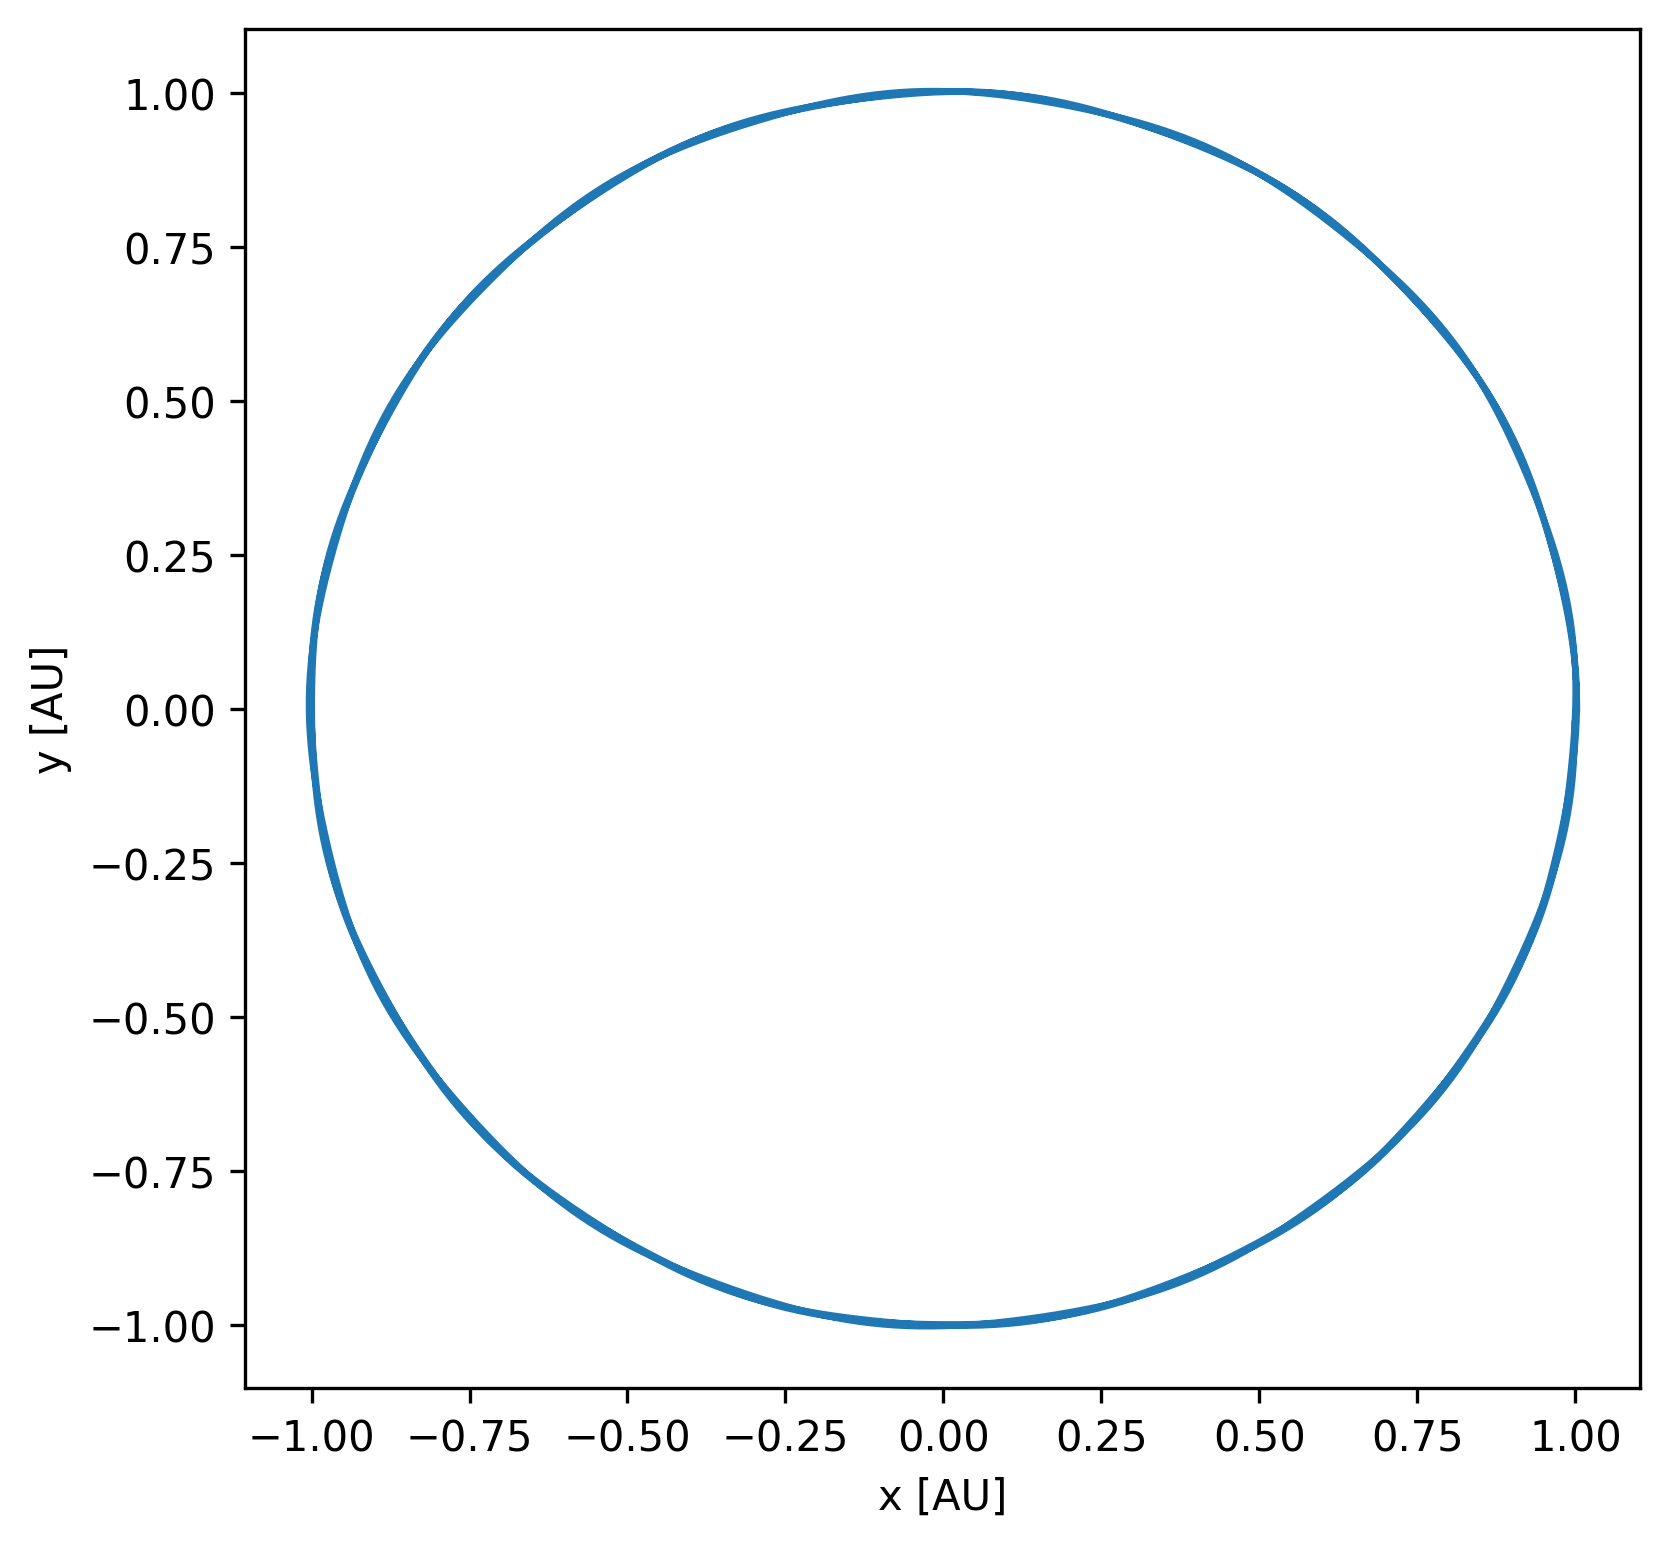
\includegraphics[width=3.5in]{homework4/1-1.png}
    \caption{Orbital trajectory over 3 years of the third (smallest) body in a 3-body system where $M_1=M_\odot$, $M_2=3\times10^{-6}M_\odot$, $M_3 = 3.7\times10^{-8}M_\odot$, $r_{12}=1$ AU, and $r_{23}= 0.0025$ AU. The calculated period of the medium-mass body (the ``planet'') is between 1.0013 and 1.0014 years.}
    \label{fig:1-1}
\end{figure}

\begin{figure}[H]
    \centering
    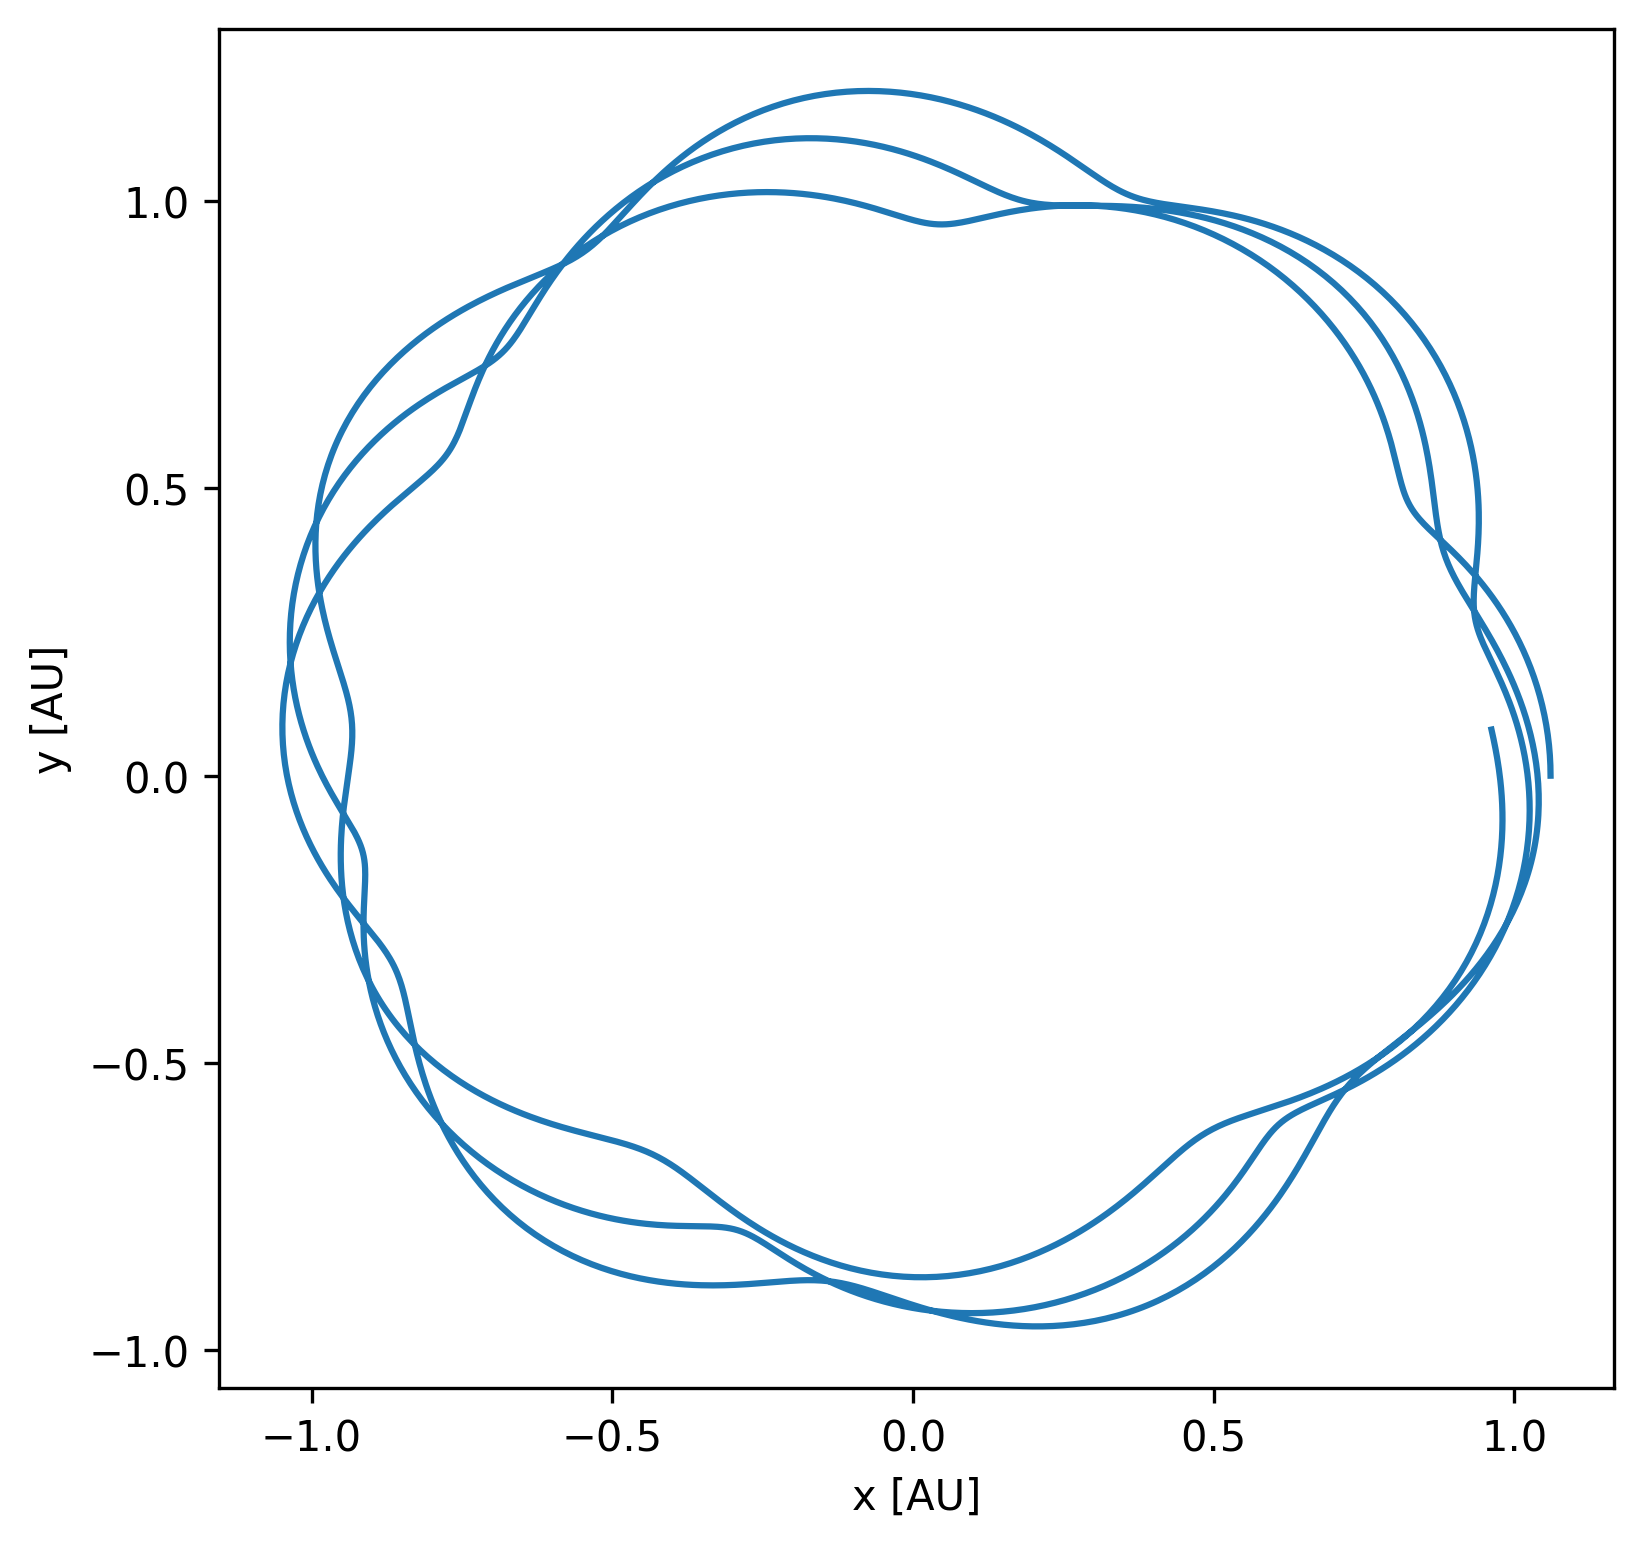
\includegraphics[width=3.5in]{homework4/1-2.png}
    \caption{Orbital trajectory over 3 years of the third (smallest) body in a 3-body system where $M_1=M_\odot$, $M_2=10^{-2}M_\odot$, $M_3 = 10^{-4}M_\odot$, $r_{12}=1$ AU, and $r_{23}= 0.0025$ AU. The calculated period of the medium-mass body (the ``planet'') is between 1.0188 and 1.0189 years.}
    \label{fig:1-2}
\end{figure}

\begin{figure}[H]
    \centering
    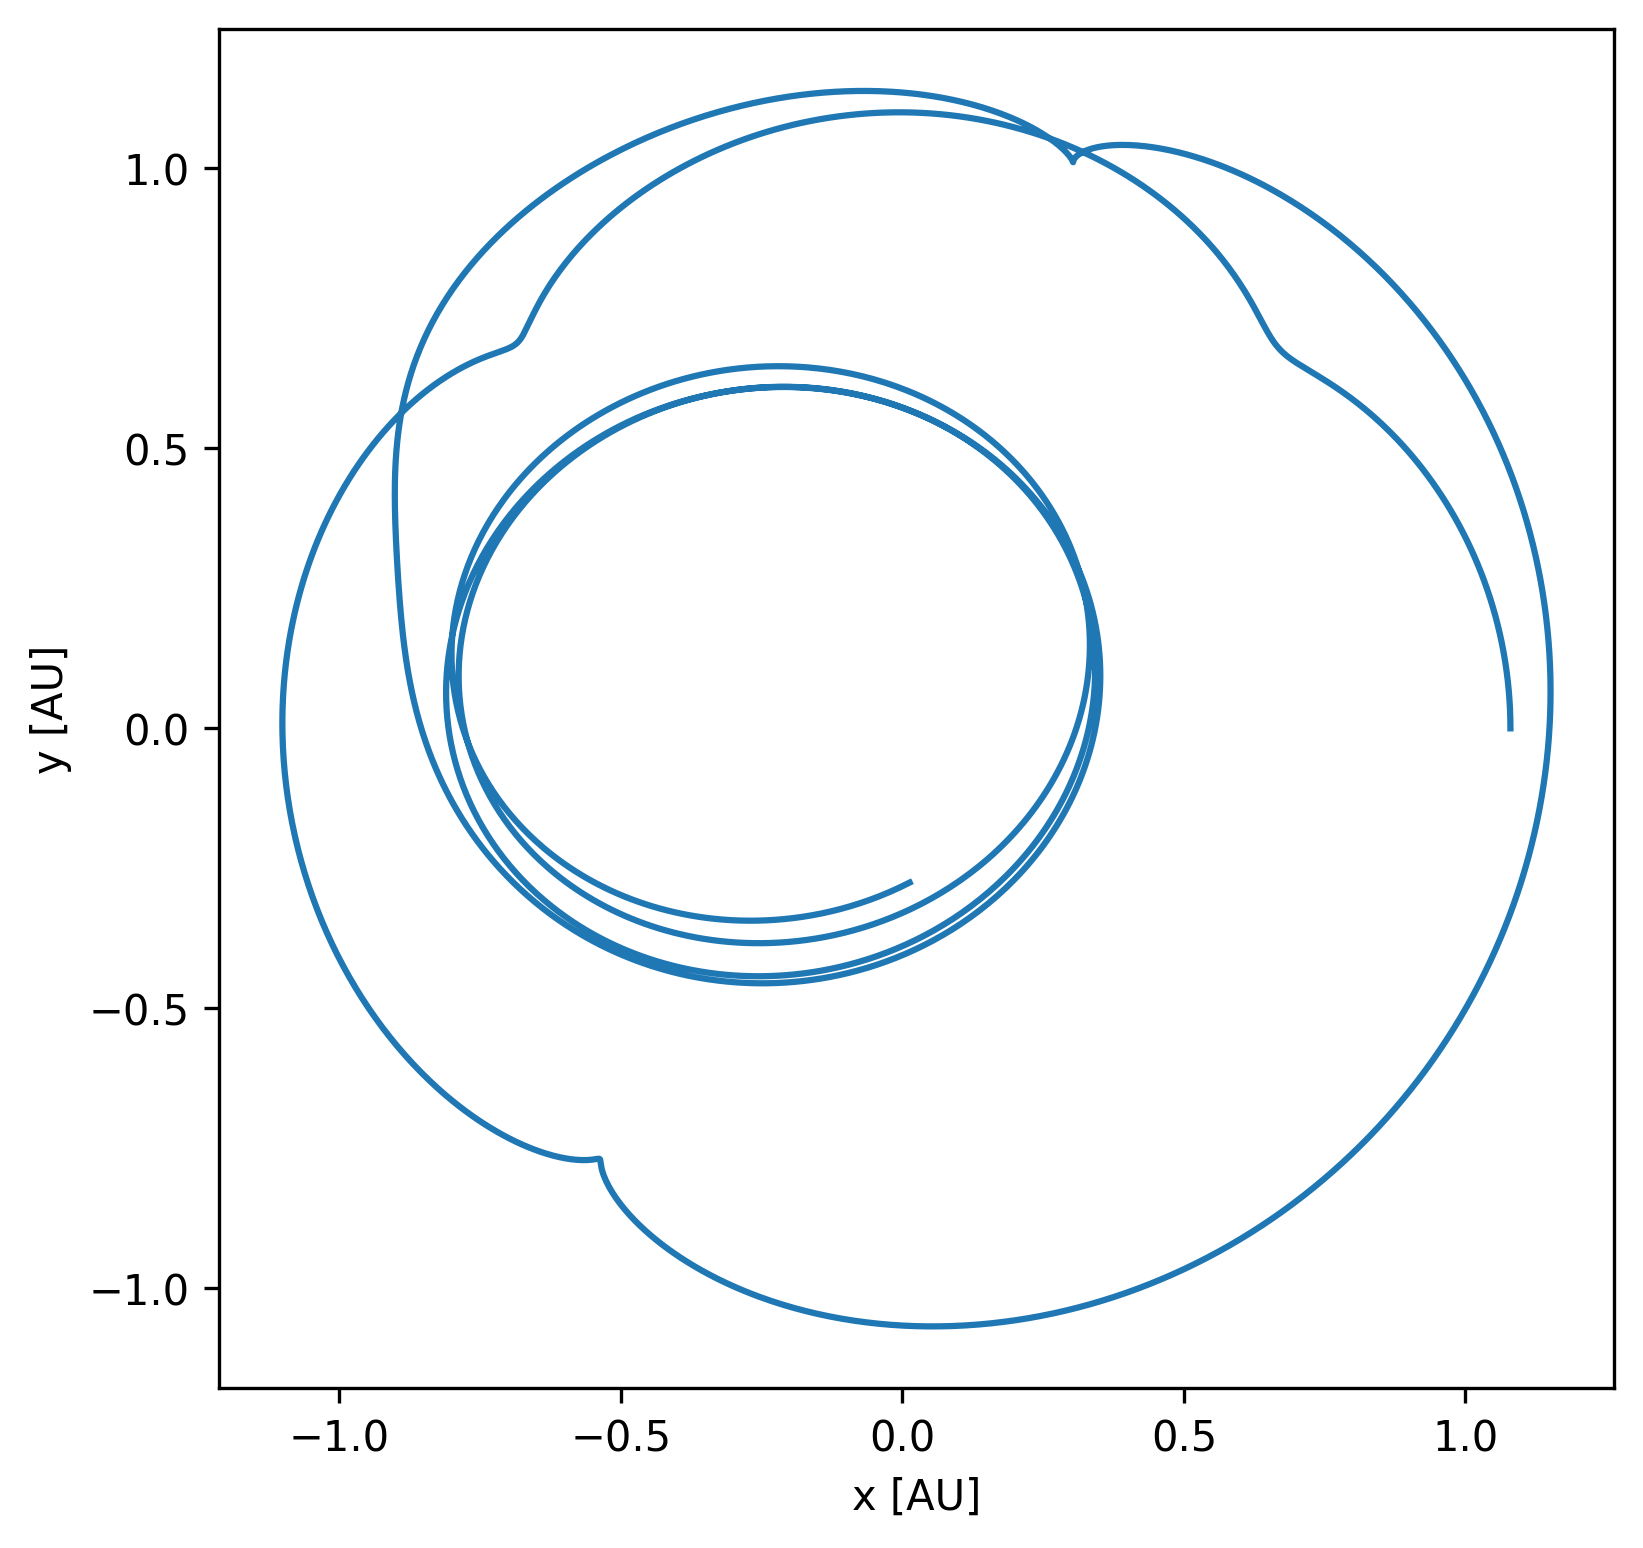
\includegraphics[width=3.5in]{homework4/1-3.png}
    \caption{Orbital trajectory over 3 years of the third (smallest) body in a 3-body system where $M_1=M_\odot$, $M_2=10^{-2}M_\odot$, $M_3 = 10^{-4}M_\odot$, $r_{12}=1$ AU, and $r_{23}= 0.08$ AU. The calculated period of the medium-mass body (the ``planet'') is between 1.0177 and 1.0178 years.}
    \label{fig:1-3}
\end{figure}

\begin{figure}[H]
    \centering
    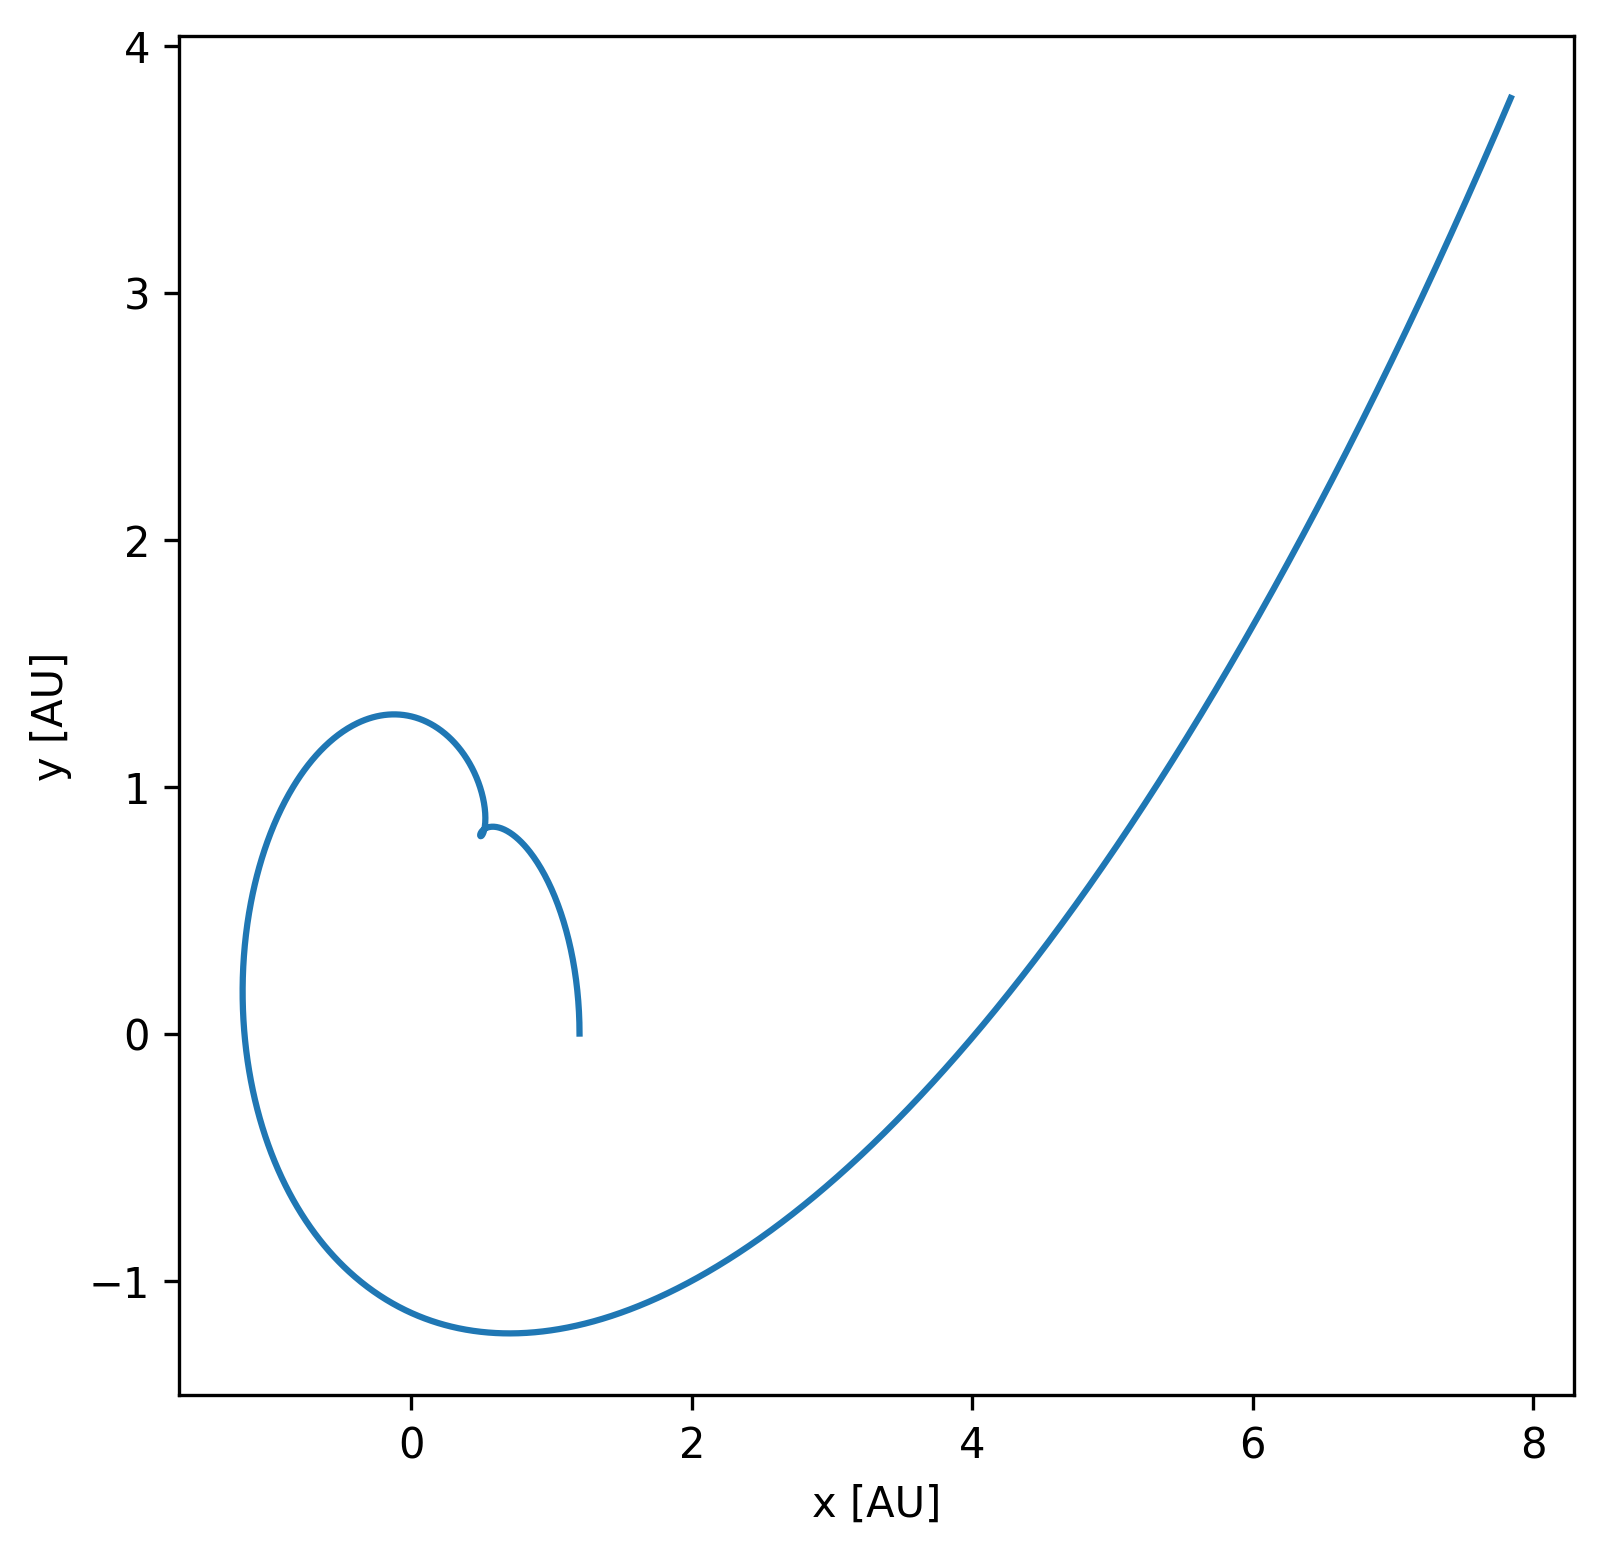
\includegraphics[width=3.5in]{homework4/1-4.png}
    \caption{Orbital trajectory over 3 years of the third (smallest) body in a 3-body system where $M_1=M_\odot$, $M_2=10^{-1}M_\odot$, $M_3 = 10^{-4}M_\odot$, $r_{12}=1$ AU, and $r_{23}= 0.2$ AU. The calculated period of the medium-mass body (the ``planet'') is between 1.0192 and 1.0193 years.}
    \label{fig:1-4}
\end{figure}

The period for the planet in each case is $\ \sim 1$ year because the initial velocities are specified such that a circular orbit will complete 1 revolution in 1 year. Changing $dt$ has little effect on these results, as the orbits for the planet are still mostly circular or elliptical, and so there is not as much accuracy to be lost in small, nuanced movements as is the case for the third, smallest body.

\bigskip
\noindent{\bf Question 2}
\medskip

\begin{figure}[H]
    \centering
    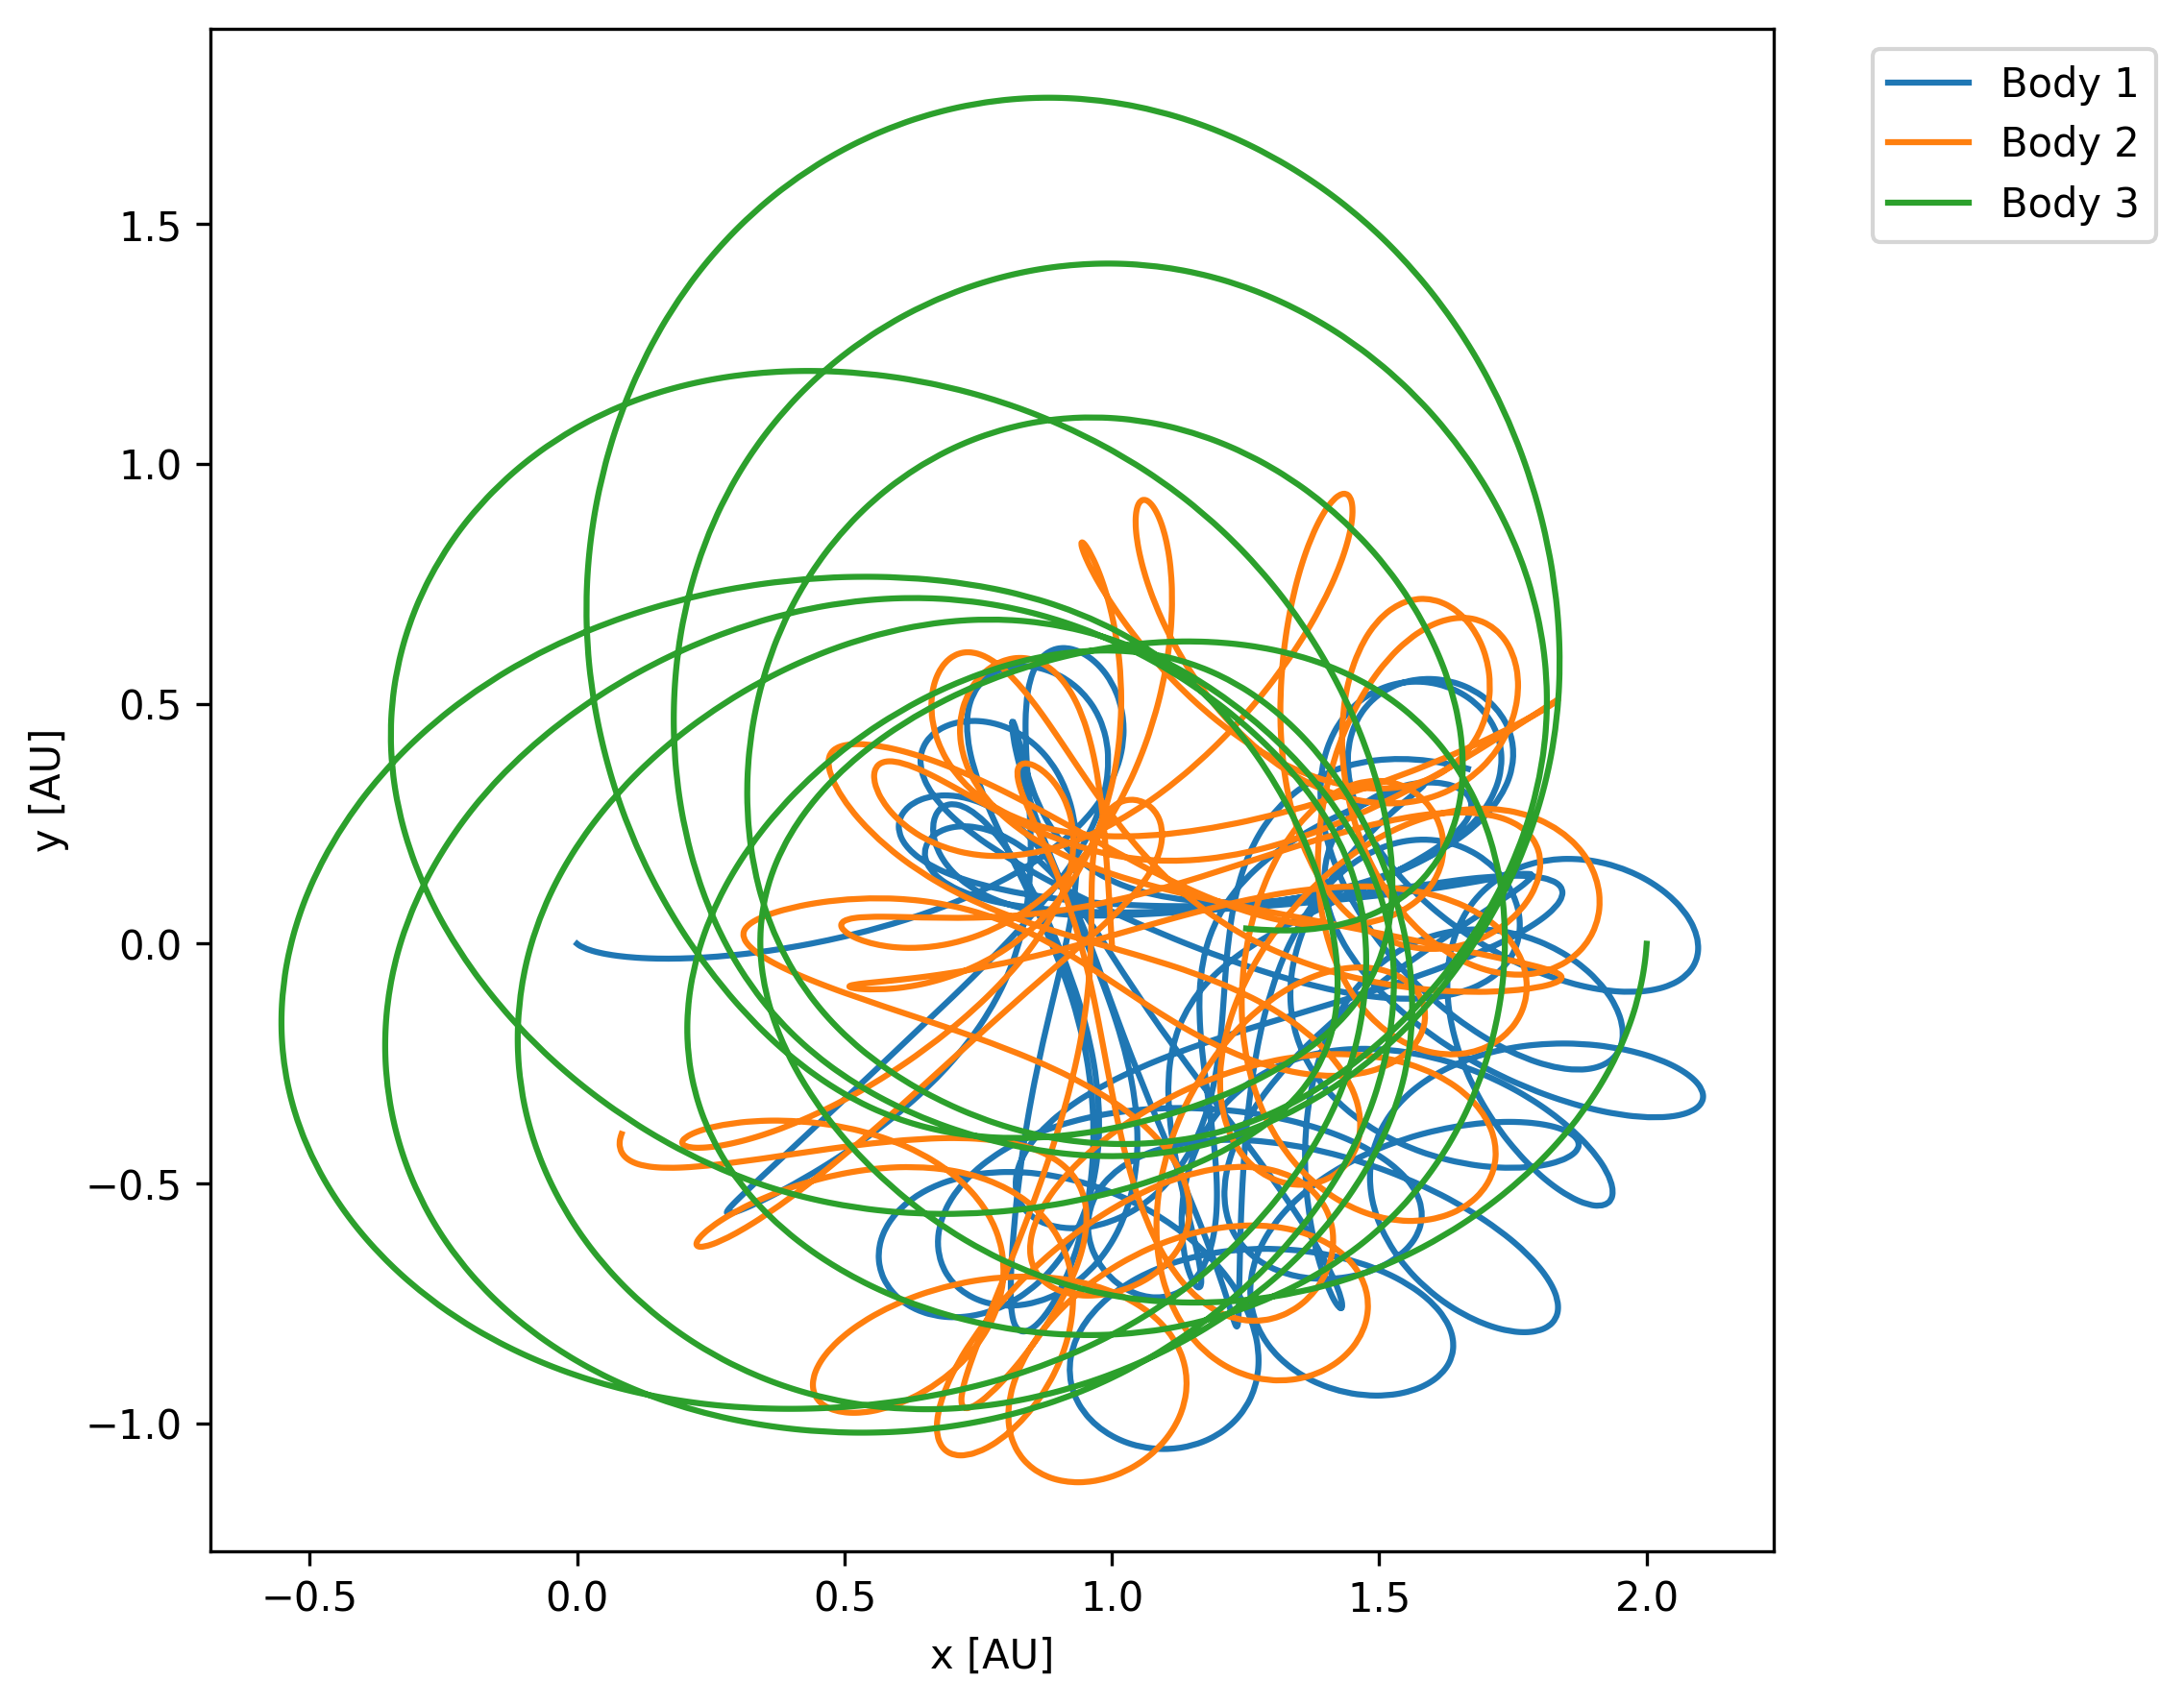
\includegraphics[width=5.5in]{homework4/p2_CM_scaled.png}
    \caption{Trajectories of three bodies over 8 years when $M_1=M_2=M_3=M_\odot$ with initial conditions satisfying $x_1 = (0,0)$ AU, $v_1 = (1,−1)$ AU/yr, $x_2 = (1,0)$ AU, $v_2 = (0,6)$ AU/yr, $x_3 = (2,0)$ AU, $v_3 = (0,−6)$ AU/yr at time $t=0$.}
    \label{fig:p2_orbits}
\end{figure}

\begin{figure}[H]
    \centering
    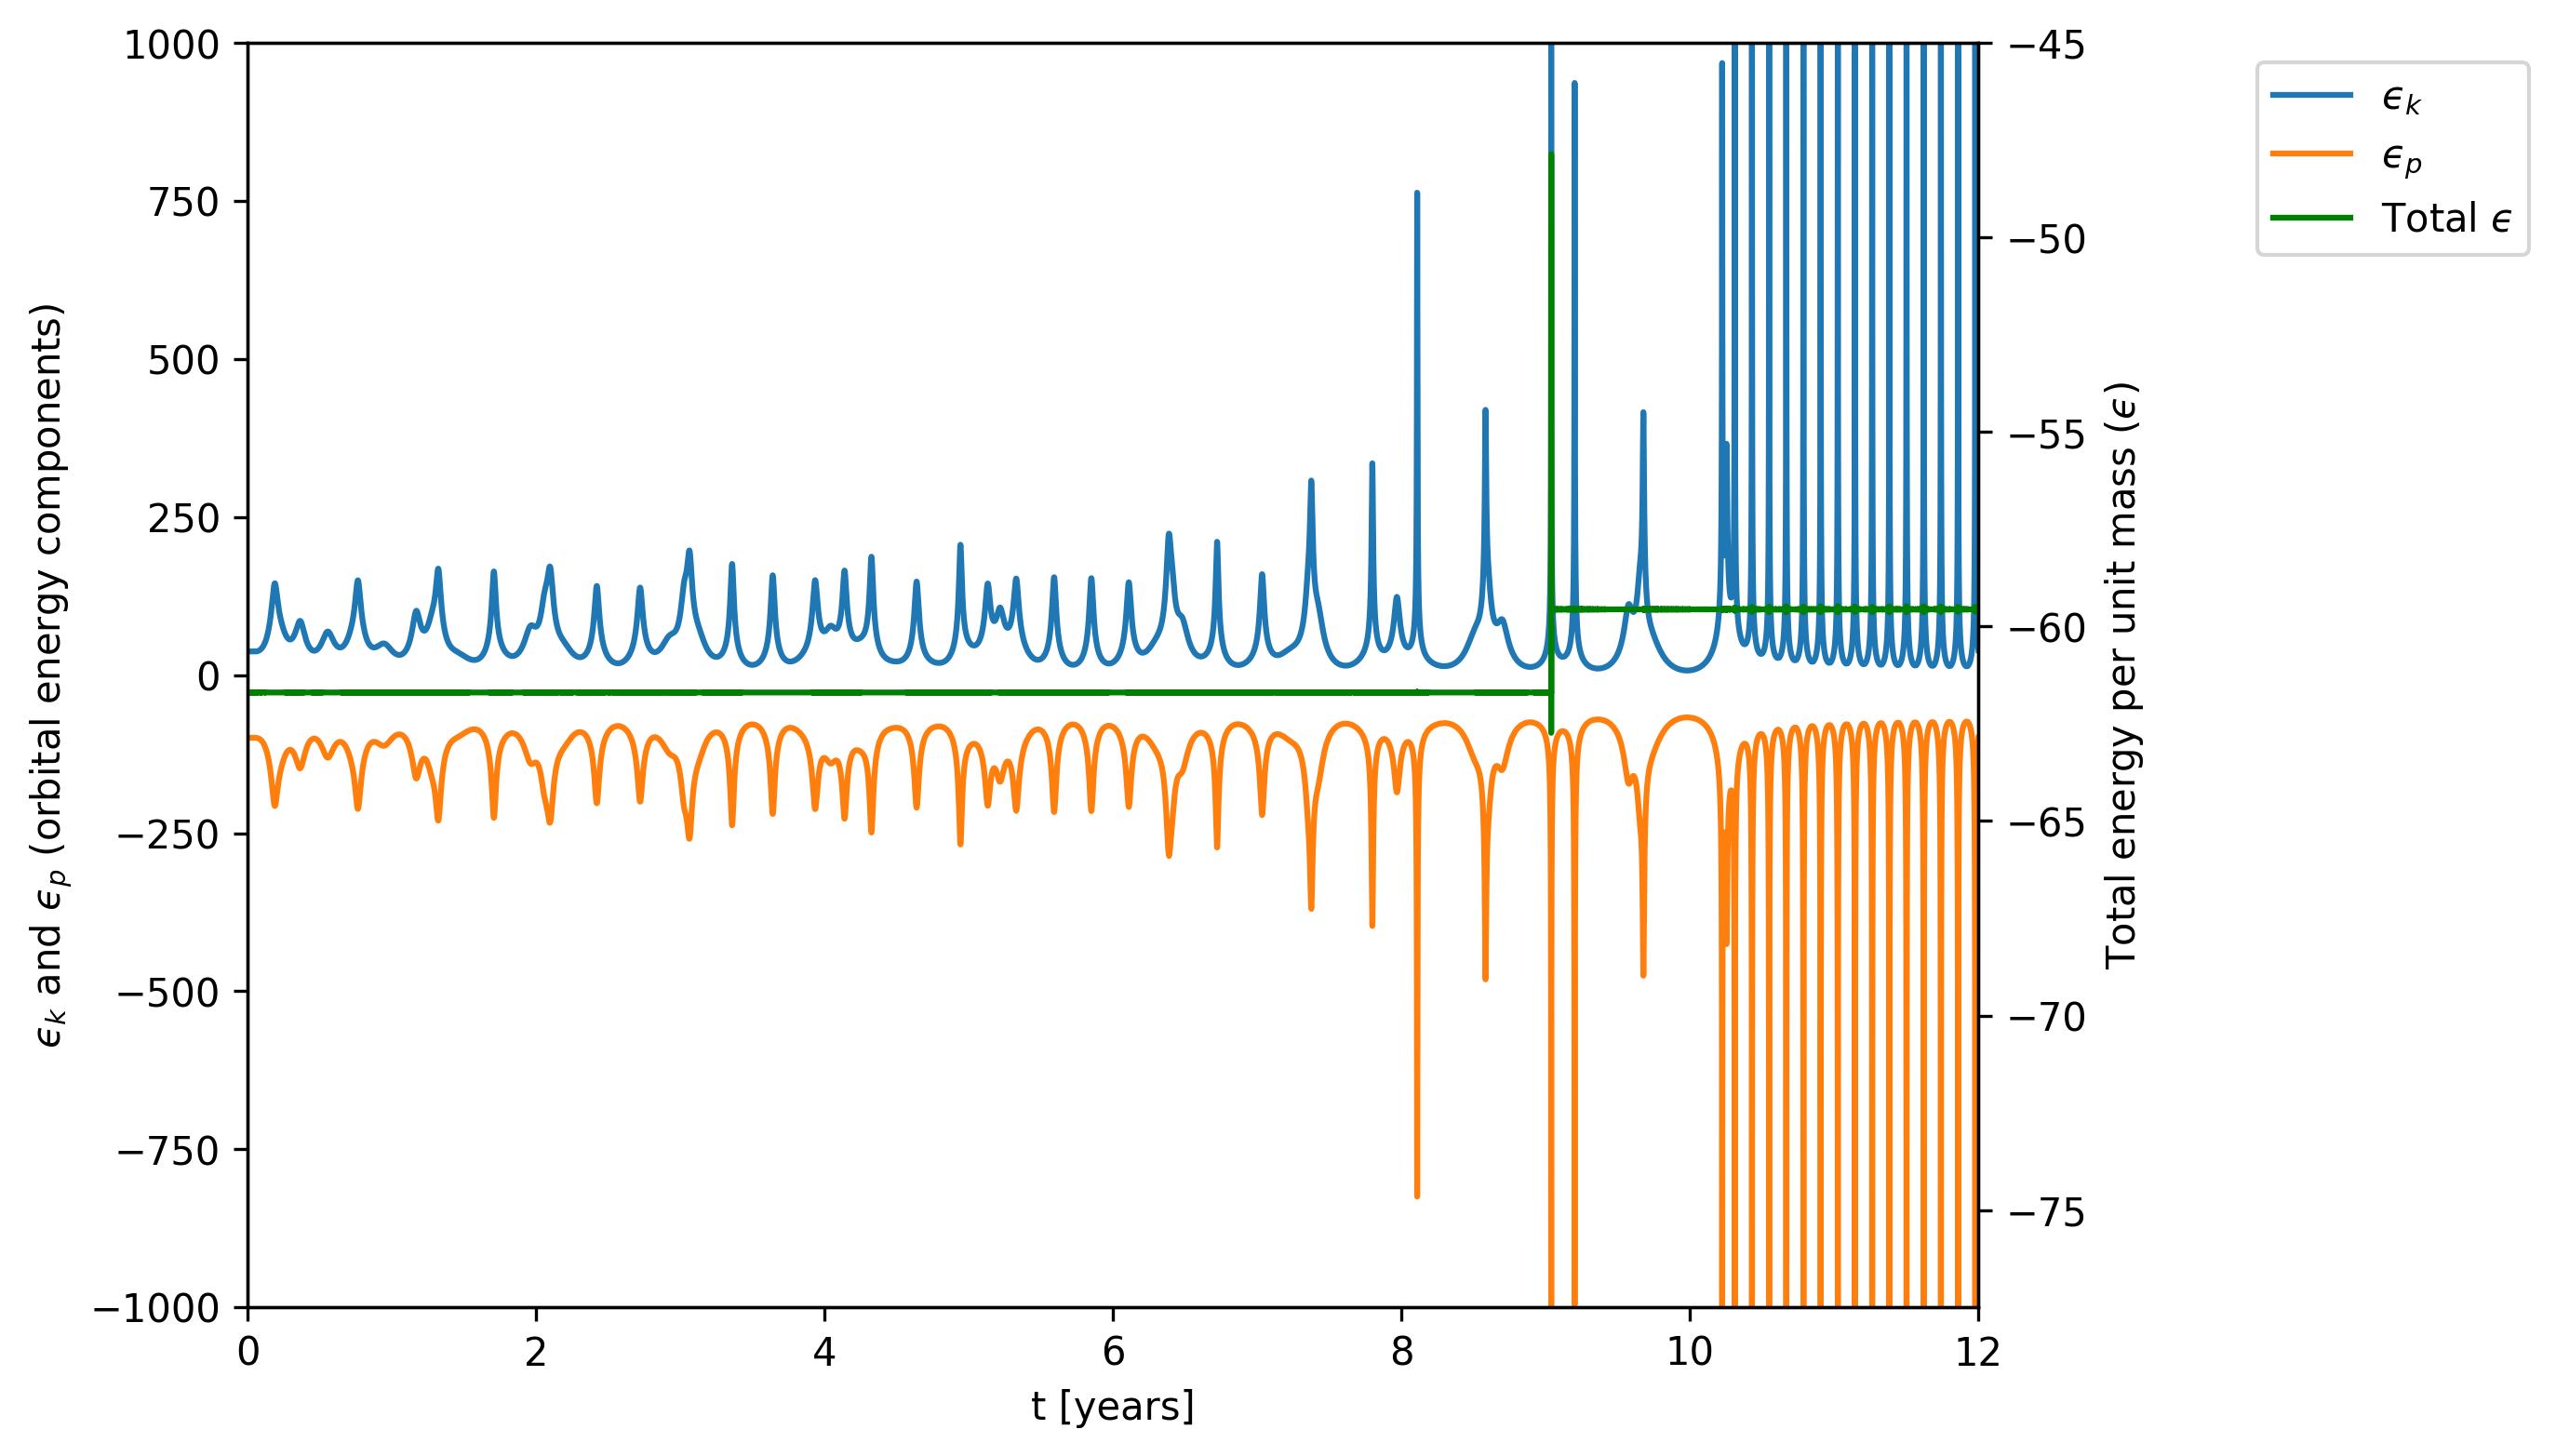
\includegraphics[width=5.5in]{homework4/q2_energy.png}
    \caption{Specific orbital energy (total energy per unit mass) breakdown of the 3-body system over 12 years. Total energy ($\epsilon_k + \epsilon_p$) remains constant, as expected, for the first $\ \sim 9$ years of the simulation, after which an obvious discontinuity occurs.}
    \label{fig:p2_energy}
\end{figure}

\begin{figure}[H]
    \centering
    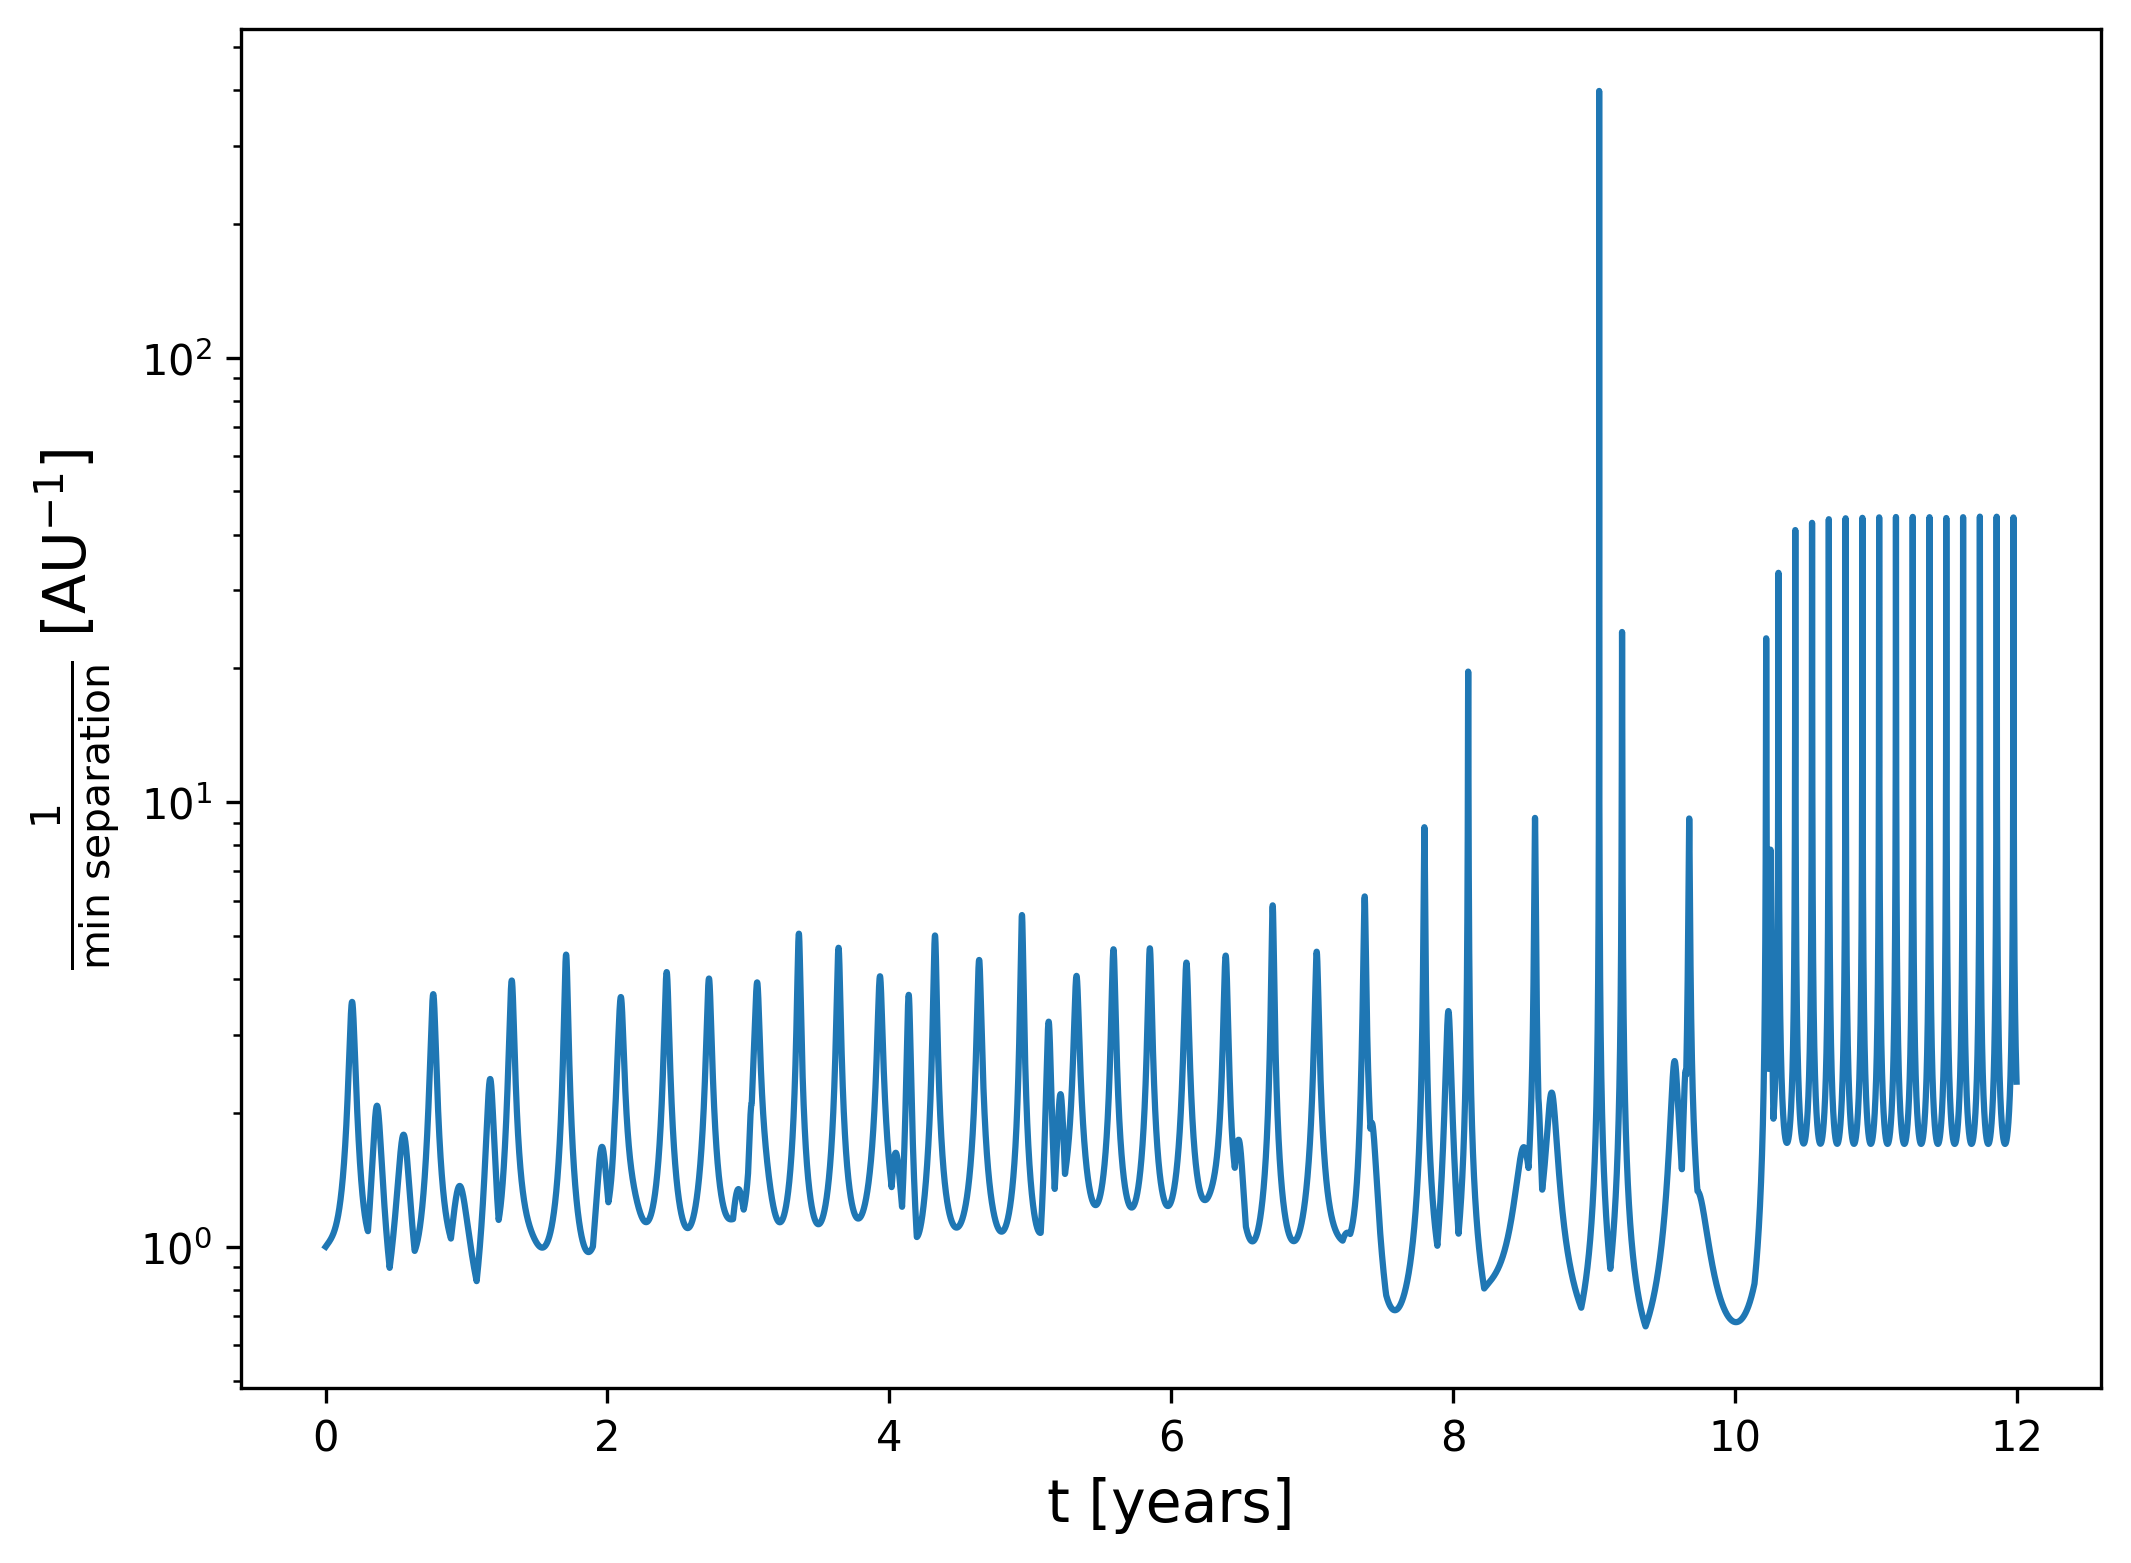
\includegraphics[width=5in]{homework4/minsep.png}
    \caption{Reciprocal of the separation between the two closest bodies at any given time over a 12-year simulation. This quantity $\frac{1}{r_\text{min}}$ is proportional to $a$, as is evident from Eq.~\ref{eq:velocity}.}
    \label{fig:minsep}
\end{figure}

\bigskip
\noindent{\bf Question 3}
\medskip

The computational complexity of performing an $N$-body simulation like this is $\mathcal{O}(N^2)$. For every new body introduced, one must run all of the calculations for each of the other bodies' relations to it. For example, a system of 2 bodies requires only one relationship to be calculated (plus the ``self''-computation, in some sense). Doubling $N$ to a 4-body system now requires computing a total of 8 interactions. Thus we observe that a doubling of $N$ results in a quadrupling ($\times N^2$) of the required computations.

\section{Conclusions}

As compared to previous assignments, I had a few more technical difficulties this time around. At first my \texttt{C} code was not functioning properly at all, and I had to scale back on some of the generalizability that I had tried to implement during the debugging process.

Additionally, the requested timestep of $dt=10^{-6}$ years is extremely computationally demanding, especially when the time domain spans 8 or 12 years. I found myself sitting idle for long periods of time simply waiting for my code to finish execution, before even knowing if the results were good or not. Additionally, the simulation results and output are at least 1--2 GB in size for some of the time domains required in this assignment. I compared the shapes of the orbits using $dt=10^{-5}$ years and $dt=10^{-6}$ years and found only minimal differences, so I hesitate to say that the marginally increased accuracy afforded by the smaller time step is worth the increased computational time.

\end{document}
